% TeX'ing this file requires that you have AMS-LaTeX 2.0 installed
% as well as the rest of the prerequisites for REVTeX 4.1
%
% See the REVTeX 4 README file
% It also requires running BibTeX. The commands are as follows:
%
%  1)  latex qde.tex
%  2)  bibtex qde
%  3)  latex qde.tex
%  4)  latex qde.tex
%
\documentclass[%
 reprint,
%superscriptaddress,
%groupedaddress,
%unsortedaddress,
%runinaddress,
%frontmatterverbose, 
%preprint,
%showpacs,preprintnumbers,
%nofootinbib,
%nobibnotes,
%bibnotes,
 amsmath,amssymb,
 aps,
 pra,
%prb,
%rmp,
%prstab,
%prstper,
%floatfix,
]{revtex4-1}

\usepackage{graphicx}% Include figure files
\usepackage{dcolumn}% Align table columns on decimal point
\usepackage{bm}% bold math
\usepackage{hyperref}% add hypertext capabilities
%\usepackage[mathlines]{lineno}% Enable numbering of text and display math
%\linenumbers\relax % Commence numbering lines

%\usepackage[showframe,%Uncomment any one of the following lines to test 
%%scale=0.7, marginratio={1:1, 2:3}, ignoreall,% default settings
%%text={7in,10in},centering,
%%margin=1.5in,
%%total={6.5in,8.75in}, top=1.2in, left=0.9in, includefoot,
%%height=10in,a5paper,hmargin={3cm,0.8in},
%]{geometry}

\usepackage{amsthm}
\newtheorem{definition}{Definition}[section]

\begin{document}

\title{Quantum Digital Signatures}

\author{Dominic Moylett}
 \email{dominic.moylett@bristol.ac.uk}
\affiliation{%
 Quantum Engineering Centre for Doctoral Training\\
 University of Bristol
}%

\date{\today}% It is always \today, today,
             %  but any date may be explicitly specified

%\pacs{Valid PACS appear here}% PACS, the Physics and Astronomy
                             % Classification Scheme.
%\keywords{Suggested keywords}%Use showkeys class option if keyword
                              %display desired
\maketitle

%\tableofcontents

\section{Introduction}
\label{sec:intro}

Cryptography studies secure communication between parties, often called Alice and Bob. In classical cryptography, this security is guaranteed through assumed hardness. RSA \cite{Rivest:1978:MOD:359340.359342}, for example, assumes that factoring integers is hard. Unfortunately, several of these problems have been proven easy in both theory \cite{Shor97} and practice \cite{MLL+12, 1604.05796} on quantum computers.

But quantum computers can also fix secrecy. Quantum Key Distribution (QKD) protocols such as BB84 \citep{BB84} can securely establish a shared key. Once Alice and Bob have a shared key, they can send messages such that an eavesdropper, Eve, cannot learn anything about their communications. This has also been demonstrated experimentally \cite{Bennett1992, Sibson:15} and now companies \footnote{\url{http://www.idquantique.com/}} offer commercial QKD.

But secrecy is only part of cryptography. Even if Alice and Bob have perfect secrecy, Eve could send a message of random gibberish to Bob pretending to be Alice. Alternatively, Eve might pretend to be Bob throughout the QKD protocol, fooling Alice into sending her message to Eve. This is one of the arguments in a white paper concluding that ``CESG does not endorse QKD for government or military applications, and advises against replacing any existing public key solutions with QKD for commercial applications'' \cite{CESG16}.

The extra precautions required to prevent these attacks are signatures. Like how someone signs a letter, a digital signature is additional data to indicate authorship. And like classical encryption, classical signatures rely on assumed hardness.

Based on the improvements in secrecy, one might ask if quantum physics can also benefit digital signatures. That is the subject of this essay. In SEC.\ \ref{sec:def}, we offer a definition of digital signatures. SEC.\ \ref{sec:lamport} describes a well-known classical digital signature, followed by quantum digital signatures (QDSs) in SEC.\ \ref{sec:qds}. Experimental results are highlighted in SEC.\ \ref{sec:experiments}. Finally, we conclude with some points of discussion.

\section{Preliminaries and Definition of Digital Signatures}
\label{sec:def}

A digital signature scheme consists of the following stages:

\begin{description}
\item[Key Generation]Alice generates a signing key and a verification key. The signing key is kept to herself, while the verification key is public.
\item[Message Signing]Alice takes a message and her signing key and produces a message-signature pair.
\item[Message Verification]Bob, takes a message-signature pair \& Alice's verification key and accepts if he thinks the message was signed by Alice.
\end{description}

For security, we care about three properties with digital signatures:

\begin{description}
\item[Honest Abort]The probability of aborting if all parties are honest is negligible.
\item[Repudiation]The probability that Alice is able to convince Bob that a message-signature pair is valid and convince another party Charlie that the same pair is invalid is negligible in terms of the security parameter.
\item[Forgery]The probability that Bob can convince someone else that a message he wrote was written by Alice is negligible in terms of the security parameter.
\end{description}

\section{Lamport's One-Time Digital Signature}
\label{sec:lamport}

The original quantum digital signature was inspired from a classical family of digital signatures by Lamport\cite{lamp79}, which use one-way functions, defined below.

\begin{definition}
Let $\mathcal{X}, \mathcal{Y}$ be arbitrary sets. A function $f:\mathcal{X} \rightarrow \mathcal{Y}$ is one-way iff $f$ can be computed in polynomial time, but for any polynomial-time randomised adversary $f^{-1}:\mathcal{Y} \rightarrow \mathcal{X}$ and uniformly selected $x \in \mathcal{X}, \mathrm{Pr}[f(f^{-1}(x)) = f(x)]$ is negligible.
\end{definition}

For a one-way function $f$, Lamport's signature is defined for an $m$-bit message below:

\begin{description}
\item[Key Generation]Alice signing key is $m$ pairs of uniformly selected integers $(k^i_0, k^i_1)$. Alice's verification key is the pairs $(f(k^i_0), f(k^i_1)), i \in \{0,...,m-1\}$.
\item[Message Signing]For each bit $m_i$ of Alice's message, she sends $k^i_{m_i}$ as her signature for that bit.
\item[Message Verification]Given Alice's verification key $\{v^i_0, v^i_1\}$ and her signature $k^i_{m_i}$, Bob accepts her message $m_i$ if $v^i_{m_i} = f(k^i_{m_i})$.
\end{description}

Because this signature scheme is classical and deterministic, recipients can compare copies of the signed message and keys, so Alice cannot repudiate.

If an attacker has two different signed messages $M, M'$ then they can construct a signature for the message $m_0m_1...m'_i...m_{m-1}$, where $m_i \neq m'_i$. So this scheme is only secure for one message. But if an adversary can forge a message given only one message from Alice, then it is possible to invert $f$, so $f$ is not one-way.

\section{Quantum Digital Signatures}
\label{sec:qds}

Note that for all of these protocols, $L$ is the security parameter, $s_a \geq 0$ is the threshold for authenticating a message from the original author, and $1 > s_v > s_a$ is the threshold for verifying a forwarded message.

\subsection{Gottesman and Chuang}

The first QDS was by Gottesman and Chuang \citep{quant-ph/0105032}. The protocol is similar to Lamport's signature scheme, but used quantum one-way functions mapping $L$-bit strings $k$ to $n$-qubit states $|f_k\rangle$. The protocol is described below, where $f$ is the quantum one-way function and $T < L/n$ is the number of copies of each key:

\begin{description}
\item[Key Generation]Alice generates pairs of $L$-bit strings $\{k^i_0, k^i_1\}, i \in \{0,...,M-1\}$ uniformly at random for her signing key. Her verification key is $(|f_{k^i_0}\rangle, |f_{k^i_1}\rangle), i \in \{0,...,M-1\}$.
\item[Message Signing]To sign a bit $b$, Alice sends $(b, k^0_b, k^1_b,...,k^{M-1}_b)$.
\item[Message Verification]To verify $(b, k^0_b, k^1_b,...,k^{M-1}_b)$, a recipient uses $f$ and SWAP tests \cite{PhysRevLett.87.167902} to determine if $|f_{k^i_b}\rangle$ matches the corresponding public key. The number of times a recipient finds that the SWAP test fails is noted as $s$. If $s \leq s_aM$ then the recipient accepts the message, and if $s > s_vM$ then the recipient rejects the message. In the case where $s_a < s \leq s_v$, the recipient concludes the message is valid but not transferable.
\end{description}

Security against forgery is possible due to Holevo's theorem \cite{Hol73}, which states that even if an eavesdropper managed to acquire all $T$ copies of the public key, they could only extract at most $Tn$ bits of data, and thus their probability of correctly guessing a single $L$-bit string of the signing key is $2^{-(L-Tn)}$. If the distance between two public keys $|\langle f_k|f_{k'}\rangle| \leq \delta$ for $k \neq k'$, then the probability of an attacker making a recipient accept a guessed signature is at most $\delta^2$. By choosing $s_v$ smaller than the probability of an adversary being accepted $(1 - \delta^2)(1 - 2^{1 - (L-Tn)})$, we ensure that each recipient most likely rejects the forgery.

It is harder to protect against repudiation, because Alice can send Bob and Charlie different states, and there is no perfect way for Bob and Charlie to check that their keys are identical. Gottesman and Chuang's solution is to introduce another step, Key Distribution, which uses a distributed SWAP test to check that the keys sent to Bob and Charlie match:

\begin{description}
\item[Key Distribution]Alice sends two copies of each key to Bob and Charlie. Bob and Charlie pick random indices $i \in \{0,...,M-1\}$ to perform a distributed SWAP on. Some of these indices they will perform SWAP tests on their own copies of the key to ensure that those match, and others Charlie will send one of his copies to Bob for a SWAP test between recipients. If enough tests fail then the protocol is aborted, otherwise the test keys are discarded and the protocol continues.
\end{description}

With this step in place, the probability of Alice being able to successfully repudiate is the probability that all distributed SWAP tests pass yet $|s_B - s_C| > (s_v - s_a)M$, where $s_B$ and $s_C$ are Bob and Charlie's incorrect counts, respectively. This probability is negligible in terms of $s_v - s_a$ and $L$.

While Lamport's signature assumes the existence of one-way functions, no such assumption is required here. This is because quantum one-way functions can be devised, such as the one by Buhrman et al.~\cite{PhysRevLett.87.167902} which leads to a negligible probability of forgery. However, there are a number of disadvantages:

\begin{enumerate}
\item Verification keys cannot be copied due to the no-cloning theorem \cite{WZ82}, so all keys must come from Alice. This requires authenticated quantum channels from Alice to each recipient, to ensure a forger doesn't simply send their own keys.
\item The recipients need to store keys in long-time quantum memory until Alice signs a message.
\item Generating and sharing a quantum one-way function is a complex task.
\item The distributed SWAP tests are not efficient.
\end{enumerate}

Over the rest of this section, we will summarise how these problems have been overcome.

\subsection{Initial Improvements}
\label{ssec:no-qmem}

Improvements were initially made by Dunjko, Wallden and Andersson \cite{PhysRevLett.112.040502}, who removed the quantum memory, the quantum SWAP test and quantum one-way functions. Their protocol for three parties is below:

\begin{description}
\item[Key Generation]Alice generates two $L$-bit keys $k^0, k^1$, which are Alice's signing keys. Alice then generates states of the form $|(-1)^{k^b_l}\alpha\rangle, l \in \{0,...,L-1\}, b \in \{0, 1\}$, where $\alpha$ is a public  positive real number and $k^b_l$ is the $l$-th bit of $k^b$. These quantum states are the verification key.
\item[Key Distribution]For two recipients, Bob and Charlie, Alice generates a copy of the above state for each participant. Bob and Charlie run their states together through a multiport (see FIG.\ \ref{fig:multiport}). For states which come out the signal port, they then use Unambiguous State Discrimination (USD) \cite{Ivanovic1987257} to distinguish the states $\{|-\alpha\rangle, |\alpha\rangle\}$, and for each unambiguous result $|(-1)^{k^b_l}\alpha\rangle$ note the value of $k^b_l$, the index $l$ and $b$.
\item[Message Signing]To sign a bit $b$, Alice sends $(b, k^b)$.
\item[Message Verification]To verify a message-signature pair $(b, k^b)$, Bob checks the bits of $k^b$ sent to him with the bits he was able to unambiguously determine, accepting if the number of mismatches is at most $s_ap_{USD}L$, where $p_{USD}$ is the USD success probability.
\end{description}

\begin{figure}
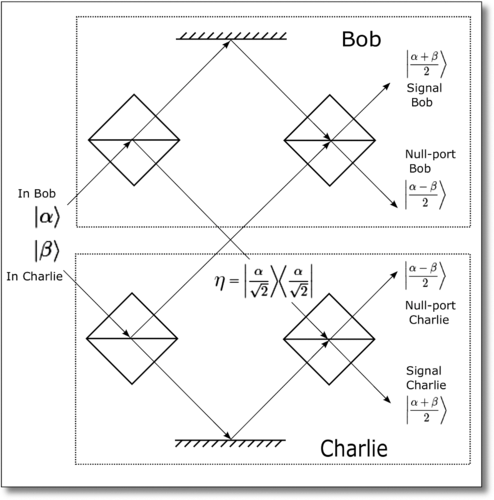
\includegraphics[width=\linewidth, natwidth=494, natheight=500]{multiport.png}
\caption{Design of a multiport. If $|\alpha\rangle = |\beta\rangle$ then $|(\alpha - \beta)/2\rangle = |0\rangle$, thus we would expect the vaccum state from the null-port. Figure from \cite{PhysRevLett.112.040502}.}
\label{fig:multiport}
\end{figure}

The multiport prevents repudiation; if Alice sends $|\alpha\rangle$ to Bob and $|\beta\rangle$ to Charlie, postselecting on photons that come out the signal outputs of the multiport ensures that both recipients have $|(\alpha + \beta)/2\rangle$. Alice's best strategy is to send a signature where the number of mismatches is halfway between the authentication and verification thresholds, which leads to her probability of repudiation being negligible in terms of $s_v - s_a$, $p_{USD}$ and $L$.

To commit forgery, Bob must guess the bits that he was not able to unambiguously determine from Alice, yet Charlie was able to. The probability of this is negligible in terms of $s_c, p_{USD}$ and $L$. Bob's other option is to send wrong states through the multiport, which Charlie can detect by aborting if too many photons are detected through his null-port.

\subsection{Quantum Digital Signatures using QKD}
\label{ssec:qds-using-qkd}

Wallden et al.\ \cite{PhysRevA.91.042304} improved the QDS by removing the multiport. This scheme uses quantum state elimination \cite{PhysRevA.89.022336} to build trust in Alice's signature. The protocol is explained below, using $|0\rangle, |1\rangle, |+\rangle = (|0\rangle + |1\rangle)/\sqrt{2}, |-\rangle = (|0\rangle - |1\rangle)/\sqrt{2}$ as the BB84 \cite{BB84} states:

\begin{description}
\item[Key Generation]Alice's signing keys are pairs $(k^0_l, k^1_l), 0 \leq l < L$ where $k \in \{0, 1, +, -\}$ is uniformly chosen. The states $\bigotimes_{l=0}^{L-1}|k^0_l\rangle$ and $\bigotimes_{l=0}^{L-1}|k^1_l\rangle$ are her verification keys.
\item[Key Distribution]Alice sends copies of the verification keys to Bob and Charlie, who pick between $L/2-r$ and $L/2+r$ indices $l \in \{0,...,L-1\}$ and bits $b \in \{0, 1\}$ for some $r$ and send $(l, b, |k^b_l\rangle)$ to each other, aborting if they receive a number outside that limit. Bob and Charlie measure all their qubits in either the $\{|0\rangle, |1\rangle\}$ or $\{|+\rangle\, |-\rangle\}$ bases, using the outcome of these measurements to note what states the key \textit{cannot} be.
\item[Message Signing]For a message $b$, Alice sends $(b, k^b_0k^b_1...k^b_{L-1})$.
\item[Message Verification]To verify $(b, k^b_0k^b_1...k^b_{L-1})$, Bob checks how many of the symbols in the signature are in the set of symbols he eliminated, accepting if this is fewer than $s_aL$.
\end{description}

Because Alice does not know which qubits Bob measured and which he forwarded to Charlie (and vice versa), she gains no repudiation advantage from sending different states to them. There is also a negligible chance of forgery; even if Bob faked the qubits he forwarded to Charlie, he would still need to guess the qubits that Charlie didn't forward to him.

\subsection{Insecure Quantum Channels}
\label{ssec:insecure-qc}

QDSs without authenticated quantum channels were proposed in two papers: one by Yin, Fu and Chen \cite{PhysRevA.93.032316} and one by Amiri et al.\ \cite{PhysRevA.93.032325}. Our focus is the latter paper.

This signature scheme uses a key generation protocol (KGP) based upon BB84 \cite{BB84}. The KGP is described below:

\begin{enumerate}
\item Bob generates $|0\rangle, |1\rangle, |+\rangle \text{ or } |-\rangle$ states and forwards these qubits to Alice.
\item Alice measures each state in either the $X$ or $Z$ basis, noting her basis and results.
\item Alice and Bob publicly announce their choice of bases and keep results that were measured in the same basis. Steps 1-3 are repeated until enough bits are produced.
\item Bob divides his key up into four parts of equal size:
\begin{itemize}
\item The first part are results from $X$ basis measurements, and will be compared with the corresponding bits from Alice.
\item The second part are results from $Z$ basis measurements, and will be compared with the corresponding bits from Alice.
\item The third part are bits that are forwarded on to Charlie.
\item The fourth part are bits that Bob keeps.
\end{itemize}
\item If there is not enough correlation or the difference in correlation between the $X$ and $Z$ measurements is too high, then the protocol is aborted.
\item Alice \& Bob discard their correlation measurement bits and Bob \& Charlie exchange their parts of the keys through a secure classical channel.
\end{enumerate}

We use this KGP to construct a QDS below:

\begin{description}
\item[Key Generation/Distribution]Bob and Charlie use the key generation protocol to generate two $L$-bit keys with Alice, half of each key being forwarded to the other party. Alice's copies of the keys are denoted $A^B_0, A^B_1, A^C_0, A^C_1$, where $B$ (resp.\ $C$) denotes Bob (resp.\ Charlie). Bob and Charlie have their own keys with Alice $B_0, B_1$ \& $C_0, C_1$ and their keys from each other $B^C_0, B^C_1$ \& $C^B_0, C^B_1$, respectively.
\item[Message Signing]To sign a bit $b$, Alice sends $(b, A^B_b, A^C_b)$.
\item[Message Verification]Given $(b, A^B_b, A^C_b)$, Bob checks the number of mismatches between $A^B_b$ \& $B_b$ and the number of mismatches between $A^C_b$ \& $B^C_b$. If the total number of mismatches is below $s_aL/2$ then the message is accepted.
\end{description}

This QDS is a more general version of protocol P2 from \cite{PhysRevA.91.042304}. While the protocol described above uses a key generation protocol that creates correlated bit strings between parties, protocol P2 uses already shared keys.

Like the protocol in SEC.\ \ref{ssec:qds-using-qkd}, security against repudiation is offered as Alice does not know which bits Bob and Charlie passed on to each other.

For Bob to forge a message, he needs to guess the bits that Charlie kept. Bob has the highest chance of success if he eavesdrops on the key generation protocol between Alice and Charlie, which he can as the quantum channel is insecure. If Bob regularly guesses the wrong qubit to forward to Alice, this will give low correlations between Alice and Charlie's measurements. When Alice and Charlie look at their correlations, they will either find low correlations in $X$ measurements or a large difference between the number of correlations in $X$ and $Z$. Either way, the protocol will be aborted.

\section{Experimental Achievements}
\label{sec:experiments}

Although there are a number of difficulties in these QDSs, experimental results have been developed with compromises. Some results are discussed below.

One of the earliest experimental results was in 2012 by Clarke et al.\ \cite{CCD+12}. This experiment encoded qubits in the phase of coherent light, created using an attenuated pulsed laser at an $850 \text{ nm}$ wavelength. The states were of the form $\{|\alpha e^{2i\pi p/N}\rangle| p = 0,1,...,N\}$, generated by a Mach-Zender interferometer with a controllable phase modulator.

Rather than implement a distributed SWAP test, Alice's pulsed laser is passed through a multiport to Bob and Charlie. A phase modulator was placed between Alice's output and Bob's multiport input to test repudiation. To avoid needing quantum memory, Bob and Charlie measured their received photons immediately using a Mach-Zender interferometer, a controllable phase modulator and Silicon Single Avalanche Photo-Diode (Si-SAPD), noting basis and result. When Alice sends her message and a classical description of the signature state, Bob and Charlie check if it is consistent with their measurements.

Clarke et al.\ saw that the gap between the probability of a successful signature for honest players and the probability of a successful forgery by Bob for their system was $8.03 \times 10^{-4} \pm 0.3 \times 10^{-4}$. The primary reasons for a gap this small were the low count rates at the detectors, which had losses of $7.5 \text{ dB}$ at the multiport null-ports and $7.1 \text{ dB}$ during measurement. The overall detection efficiency ranged from $36-42\%$.

A later paper by Collins et al.\ \cite{PhysRevLett.113.040502} implemented the signature from SEC.\ \ref{ssec:no-qmem}. This experiment largely used the same setup as \cite{CCD+12}, but Bob and Charlie's measurements now used two Mach-Zender interferometers separated by a beamsplitter: one to measure $\{|\alpha\rangle, |\alpha e^{i\pi}\rangle\}$ and one to measure $\{|\alpha e^{i\pi/2}\rangle, |\alpha e^{3i\pi/2}\rangle\}$, which were the qubit encodings used by Alice. Another difference is that Collins et al.\ used unambiguous state elimination instead of USD.

Sadly, the gap was even smaller, at most $1.2 \time 10^{-6}$. For this protocol to fail with probability at most $0.01\%$ when signing a one-bit message, this would require a verification key of $5.1 \times 10^{13}$ qubits. To reduce this number, suggestions made by the authors include finding optimal photon numbers for state elimination, switching to protocols that do not require a multiport, and increasing clock speeds.

The final paper was by Donaldson et al.\ \cite{PhysRevA.93.012329}, where they demonstrated a QDS across $500-2000\text{ m}$ of fibre. The distance limitations with the previous experiments were caused by the multiport, which restricted the transmission distance to $5\text{ m}$. In this paper, the multiport is removed and repudiation is prevented by Bob \& Charlie taking measurements and forwarding the results to each other.

When the sender and receiver were separated by $500 \text{ m}$ of fibre, the gap was at most $2.86 \times 10^{-4}$. For a failure probability of at most 0.01\%, this requires a signature of $1.93 \times 10^{9}$ qubits. At the $100 \text{ MHz}$ pulse rate this experiment was operating at, one signature would take approximately $20 \text{ s}$. This signature length increased as the distance increased, but at $2000\text{ m}$ was still four orders of magnitude smaller than what was required in \cite{PhysRevLett.113.040502}. But this is still not on par with QKD or classical signatures. Suggested improvements include changing to $1550 \text{ nm}$ wavelength lasers, which have lower losses in telecommunications fibres -- $0.2\text{ dB km}^{-1}$ instead of $2.2\text{ dB km}^{-1}$ -- as well as better detectors, such as semiconductor \cite{0957-0233-21-1-012002} or even superconducting \cite{0953-2048-25-6-063001} detectors.

\section{Conclusion and Discussion}
\label{sec:conclusion}

To quote the CESG white paper again \cite{CESG16}, ``modern services [...] rely more on authentication and integrity mechanisms, such as digital signatures, than on encryption.'' While quantum key distribution has the potential to be significantly beneficial over classical encryption alone, secrecy alone is not enough.

Despite only being proposed in 2001, QDSs have come a long way. Gottesman and Chuang's original scheme \cite{quant-ph/0105032} had many practical limitations, but many of these have now been fixed, particularly following the work of Yin, Fu and Chen \cite{PhysRevA.93.032316} and Amiri et al.\ \cite{PhysRevA.93.032325}. But there are still limitations: While both protocols do not require quantum channel authentication, Amiri et al.'s is still dependent on authenticated classical channels, and it is unknown how to make Yin, Fu and Chen's scale with participants, particularly in order to prevent collusion attacks.

Experimentally, proof of principle QDSs have been demonstrated using phase-encoded coherent states of light over growing distances. However, the length of keys required in order to currently provide safe levels of security is impractical, taking $20\text{ s}$ to generate the keys for signing and verifying a single bit. By incorporating advances in optical devices such as improved single photon detectors, QDSs will hopefully advance further towards being on par with QKD.

Finally, it is worth noting one more weakness of QDSs: They are only secure for signing a single message. This means that all of the (quantum and classical) communication to establish keys must be repeated for every single bit. Classically, such overhead is avoided by using signatures which reuse keys, such as the Digital Signature Algorithm \cite{kravitz1993digital}. Such a property is sadly not trivial, if possible, in quantum digital signatures.

\bibliography{qde}% Produces the bibliography via BibTeX.

\appendix

\end{document}
%
% ****** End of file qde.tex ******
